\section{AD Functionality}
\subsection{Flexible Signle Master Operation roles}
In the early days of AD, if you had multiple DCs in an environment, they would fight over which DC gets to make changes, and sometimes changes would not be made properly.
Microsoft then implemented "last writer wins," which could introduce its own
problems if the last change breaks things. They then introduced a model in
which a single "master" DC could apply changes to the domain while the others merely fulfilled authentication requests. This was a flawed design because
if the master DC went down, no changes could be made to the environment
until it was restored. To resolve this single point of failure model, Microsoft
separated the various responsibilities that a DC can have into \gls{win:FSMO}.

These give Domain Controllers (DC) the ability to continue authenticating users and granting permissions without interruption (authorization and authentication). There are five FMSO roles:

\begin{tabularx}{\linewidth}{|l|X|}
    \hline
Roles & Description \\
    \hline
Schema Master & This role manages the read/write copy of the \gls{win:schema}, which
defines all attributes that can apply to an object in AD.\\
    \hline
Domain Naming Master & Manages domain names and ensures that two domains of
the same name are not created in the same forest. \\
    \hline
Relative ID (RID) Master & The RID Master assigns blocks of RIDs to other DCs
within the domain that can be used for new objects. The RID Master helps ensure
that multiple objects are not assigned the same SID. Domain object SIDs are the
domain SID combined with the RID number assigned to the object to make the
unique SID. \\
    \hline
PDC Emulator & The host with this role would be the authoritative DC in the
domain and respond to authentication requests, password changes, and manage
Group Policy Objects (GPOs). The PDC Emulator also maintains time within the
domain. \\
    \hline
Infrastructure Master & This role translates GUIDs, SIDs, and DNs between
domains. This role is used in organizations with multiple domains in a single
forest. The Infrastructure Master helps them to communicate. If this role is
not functioning properly, Access Control Lists (ACLs) will show SIDs instead of
fully resolved names. \\
    \hline
\end{tabularx}


All five roles are assigned to the first DC in the forest root domain in a new AD forest. Each time a new domain is added to a forest, only the RID Master, PDC Emulator, and Infrastructure Master roles are assigned to the new domain. 

FSMO roles are typically set when domain controllers are created, but sysadmins can transfer these roles if needed. These roles help replication in AD to run smoothly and ensure that critical services are operating correctly.  We will walk through each of these roles in detail later in this section.

\subsection{Domain and Forest Functional Levels}

functional levels determine the various  features and capabilities available in Active Directory Domain Services  (AD DS) at the domain and forest level. They are also used to specify  which Windows Server operating systems can run a Domain Controller in a  domain or forest. 

\subsubsection{Domain functional level features}
\begin{tabularx}{\linewidth}{|l|X|}
    \hline
Domain Functional Level & Features Available \\
    \hline
Windows 2000 native & Universal groups for distribution and security groups,
group nesting, group conversion (between security and distribution and security
groups), SID history. \\
    \hline
Windows Server 2003 & Netdom.exe domain management tool, lastLogonTimestamp
attribute introduced, well-known users and computers containers, constrained
delegation, selective authentication. \\
    \hline
Windows Server 2008 & Distributed File System (DFS) replication support,
Advanced Encryption Standard (AES 128 and AES 256) support for the Kerberos
protocol, Fine-grained password policies \\
    \hline
Windows Server 2008 R2 & Authentication mechanism assurance, Managed Service
Accounts \\
    \hline
Windows Server 2012 & KDC support for claims, compound authentication, and
Kerberos armoring \\ 
    \hline
Windows Server 2012 R2 & Extra protections for members of the Protected Users
group, Authentication Policies, Authentication Policy Silos \\
    \hline
Windows Server 2016 & Smart card required for interactive logon new Kerberos
features and new credential protection features \\
    \hline
\end{tabularx}


\subsubsection{Forest functional level features}
\begin{tabularx}{\linewidth}{|l|X|}
    \hline
Version & Capabilities \\
    \hline
Windows Server 2003 & saw the introduction of the forest trust, domain
renaming, read-only domain controllers (RODC), and more. \\
    \hline
Windows Server 2008 & All new domains added to the forest default to the
Server 2008 domain functional level. No additional new features. \\
    \hline
Windows Server 2008 R2 & Active Directory Recycle Bin provides the ability to
restore deleted objects when AD DS is running. \\
    \hline
Windows Server 2012 & All new domains added to the forest default to the
Server 2012 domain functional level. No additional new features. \\
    \hline
Windows Server 2012 R2 & All new domains added to the forest default to the
Server 2012 R2 domain functional level. No additional new features. \\
    \hline
Windows Server 2016 & Privileged access management (PAM) using Microsoft
Identity Manager (MIM). \\
    \hline

\end{tabularx}

\subsection{Trusts}
\label{active-directory:trust}

An Active Directory (AD) Forest is the security and administrative boundary for
objects and entities.
\href{https://social.technet.microsoft.com/wiki/contents/articles/50969.active-directory-forest-trust-attention-points.aspx}{trust}
is used to establish \verb+forest-forest+ or \verb+domain-domain+
authentication, allowing users to access resources in (or administer)  another
domain outside of the domain their account resides in. A trust  creates a link
between the authentication systems of two domains.

There are several trust types:

\begin{tabularx}{\linewidth}{|l|X|}
    \hline
Trust Type & Description \\
    \hline
Parent-child & Domains within the same forest. The child domain has a two-way
transitive trust with the parent domain. \\
    \hline
Cross-link & a trust between child domains to speed up authentication. \\
    \hline
External & A non-transitive trust between two separate domains in separate
forests which are not already joined by a forest trust. This type of trust
utilizes
\href{https://www.serverbrain.org/active-directory-2008/sid-history-and-sid-filtering.html}{SID
filtering}. \\
    \hline
Tree-root & a two-way transitive trust between a forest root domain and a new
tree root domain. They are created by design when you set up a new tree root
domain within a forest. \\
    \hline
Forest & a transitive trust between two forest root domains.\\ 
    \hline
\href{https://docs.microsoft.com/en-us/security/compass/esae-retirement}{ESAE}
    & A bastion forest used to manage Active Directory which is becoming
    obsolete\\
\end{tabularx}

\begin{figure}
  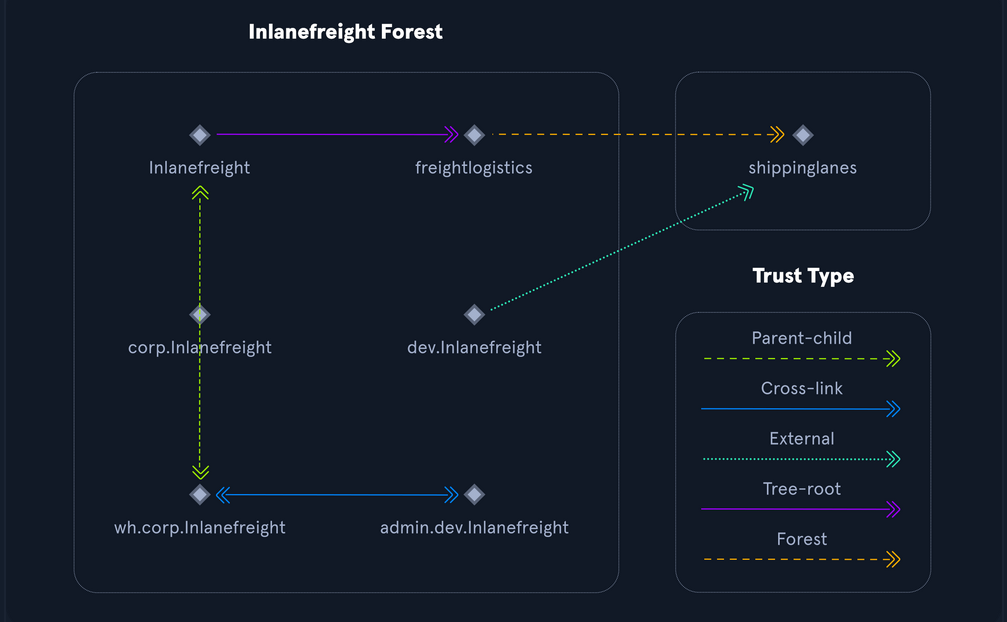
\includegraphics[width=\linewidth]{windows_knowledge/ad/images/trusts.png}
  \caption{AD trusts}
  \label{fig:ad-trusts}
\end{figure}

Trusts can be:
\begin{itemize}
\item transitive: trust is extended to objects that the child domain trusts.
\item non-transitive: only the child domain itself is trusted.
\end{itemize}


Trusts can be set up:
\begin{itemize}
    \item bidirectional: users from both trusting domains can access resources.
    \item In a one-way trust: only users in a trusted domain can access resources in a trusting domain, not vice-versa. The direction of trust is opposite to the direction of access.
\end{itemize}

Often, domain trusts are set up improperly and provide unintended  attack
paths. Also, trusts set up for ease of use may not be reviewed  later for
potential security implications. Mergers and acquisitions can  result in
bidirectional trusts with acquired companies, unknowingly  introducing risk
into the acquiring company's environment. It is not  uncommon to be able to perform an attack such as Kerberoasting against a  domain outside the principal domain and obtain a user that has  administrative access within the principal domain.
